%%%%%%%%%%%%%%%%%%%%%%%%%%%%%%%%%%%%%%%%%
% Beamer Presentation
% LaTeX Template
% Version 1.0 (10/11/12)
%
% This template has been downloaded from:
% http://www.LaTeXTemplates.com
%
% License:
% CC BY-NC-SA 3.0 (http://creativecommons.org/licenses/by-nc-sa/3.0/)
%
%%%%%%%%%%%%%%%%%%%%%%%%%%%%%%%%%%%%%%%%%

%----------------------------------------------------------------------------------------
%   PACKAGES AND THEMES
%----------------------------------------------------------------------------------------

\documentclass{beamer}

\mode<presentation> {

% The Beamer class comes with a number of default slide themes
% which change the colors and layouts of slides. Below this is a list
% of all the themes, uncomment each in turn to see what they look like.

%\usetheme{default}
%\usetheme{AnnArbor}
%\usetheme{Antibes}
%\usetheme{Bergen}
%\usetheme{Berkeley}
%\usetheme{Berlin}
%\usetheme{Boadilla}
%\usetheme{CambridgeUS}
%\usetheme{Copenhagen}
%\usetheme{Darmstadt}
%\usetheme{Dresden}
%\usetheme{Frankfurt}
%\usetheme{Goettingen}
%\usetheme{Hannover}
%\usetheme{Ilmenau}
%\usetheme{JuanLesPins}
\usetheme{Luebeck}
%\usetheme{Madrid}
%\usetheme{Malmoe}
%\usetheme{Marburg}
%\usetheme{Montpellier}
%\usetheme{PaloAlto}
%\usetheme{Pittsburgh}
%\usetheme{Rochester}
%\usetheme{Singapore}
%\usetheme{Szeged}
%\usetheme{Warsaw}

% As well as themes, the Beamer class has a number of color themes
% for any slide theme. Uncomment each of these in turn to see how it
% changes the colors of your current slide theme.

%\usecolortheme{albatross}
%\usecolortheme{beaver}
%\usecolortheme{beetle}
%\usecolortheme{crane}
%\usecolortheme{dolphin}
%\usecolortheme{dove}
%\usecolortheme{fly}
%\usecolortheme{lily}
%\usecolortheme{orchid}
%\usecolortheme{rose}
\usecolortheme{seagull}
%\usecolortheme{seahorse}
%\usecolortheme{whale}
%\usecolortheme{wolverine}

%\setbeamertemplate{footline} % To remove the footer line in all slides uncomment this line
%\setbeamertemplate{footline}[page number] % To replace the footer line in all slides with a simple slide count uncomment this line

%\setbeamertemplate{navigation symbols}{} % To remove the navigation symbols from the bottom of all slides uncomment this line
}

\usepackage{graphicx} % Allows including images
\usepackage{booktabs} % Allows the use of \toprule, \midrule and \bottomrule in tables
\usepackage{verbatim}

\usepackage{color}

\newcommand{\vimmode}[1]{\texttt{#1}}

\newcommand{\viminsert}[1]{\texttt{\textcolor{blue}{#1}}}
\newcommand{\vimnormal}[1]{\texttt{\textcolor{orange}{#1}}}
\newcommand{\vimcommand}[1]{\texttt{\textcolor{brown}{#1}}}
\newcommand{\vimvisual}[1]{\texttt{\textcolor{purple}{#1}}}
\newcommand{\vimrc}[1]{\texttt{\textcolor{brown}{#1}}}

\newcommand{\vimoperator}[1]{\texttt{\textcolor{orange}{#1}}}
\newcommand{\vimmotion}[1]{\texttt{\textcolor{orange}{#1}}}

\newcommand{\vimhelp}[1]{\vimcommand{:h #1}}

\newcommand{\vimkey}[1]{\textless{}#1\textgreater{}}

%----------------------------------------------------------------------------------------
%   TITLE PAGE
%----------------------------------------------------------------------------------------

\title[Vim Intro]{Comprehensive presentation of Vim features} % The short title appears at the bottom of every slide, the full title is only on the title page

\author{Aleksander Gajewski} % Your name
\institute[None] % Your institution as it will appear on the bottom of every slide, may be shorthand to save space
{
\textit{adiog@brainfuck.pl} % Your email address
}
\date{\today} % Date, can be changed to a custom date

\begin{document}

\begin{frame}
\titlepage % Print the title page as the first slide
\end{frame}

\begin{frame}
    \frametitle{Overview}
    Vim is a highly customizable, modal editor. It is extensible with built-in vimscript language, python-support and huge collection of plugins.\\
    This presentation is intended to give a general overview of Vim and be a first reference for a novice user to start using its feature efficiently.\\
    For futher information please
    \begin{enumerate} 
        \item use vim internal help (:h \textrm{*topic*})
        \item run vimtutor
        \item visit vimcasts.org
        \item visit learnvimscriptinahardway.com
        \item visit stackoverflow.com/tag/vim
    \end{enumerate}
\end{frame}

\begin{frame}[fragile]
    \frametitle{Vi Improved}
    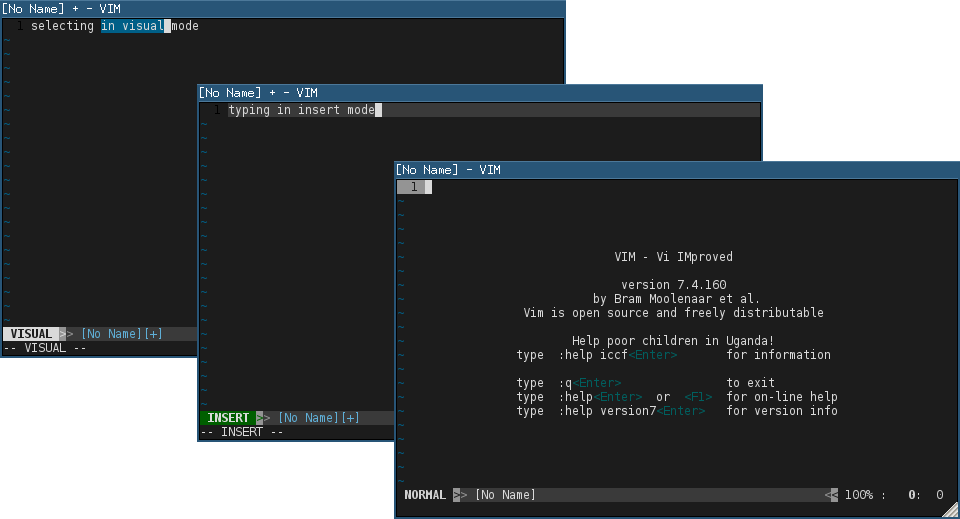
\includegraphics[width=\textwidth]{vim_screen.png}
\end{frame}

\begin{frame}[fragile]
    \frametitle{Modes overview \vimhelp{vim-modes}}
    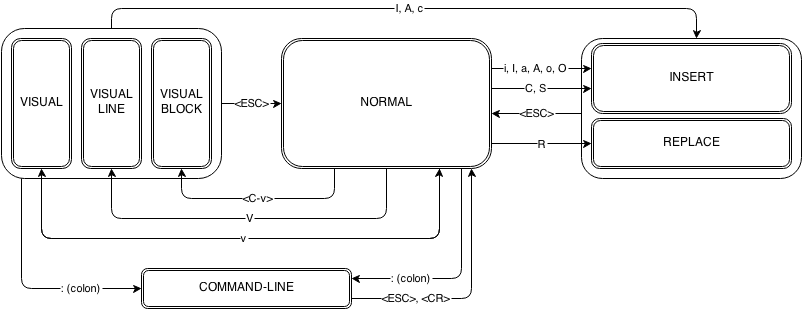
\includegraphics[width=\textwidth]{vim_modes.png}
\end{frame}

\begin{frame}[fragile]
    \frametitle{Notation}
    To avoid confusion the following colors will be used to indicate the initial modes of key sequence:
    \begin{itemize}
        \item \vimnormal{\vimmode{normal}} $\rightarrow$ \viminsert{\vimmode{insert}}: \vimnormal{i}, \vimnormal{I}, \vimnormal{a}, \vimnormal{A}, \vimnormal{o}, \vimnormal{O}, \vimnormal{C}, \vimnormal{S}
        \item \vimvisual{\vimmode{visual}} $\rightarrow$ \viminsert{\vimmode{insert}}: \vimvisual{I}, \vimvisual{A}, \vimvisual{c}
        \item \vimvisual{\vimmode{visual}} $\rightarrow$ \vimnormal{\vimmode{normal}}: \vimvisual{\vimkey{ESC}}
        \item \viminsert{\vimmode{insert}} $\rightarrow$ \vimnormal{\vimmode{normal}}: \viminsert{\vimkey{ESC}}
        \item \vimnormal{\vimmode{normal}} $\rightarrow$ \vimvisual{\vimmode{visual}}: \vimnormal{v}, \vimnormal{V}, \vimnormal{\vimkey{C-v}}
        \item \vimnormal{\vimmode{normal}} $\rightarrow$ \vimcommand{command}: \vimnormal{:}
        \item \vimvisual{\vimmode{visual}} $\rightarrow$ \vimcommand{command}: \vimnormal{:} (\vimcommand{:'\textless{},'\textgreater{}} indicates visual range) 
        \item \vimcommand{command} $\rightarrow$ \vimnormal{\vimmode{normal}}: \vimcommand{\vimkey{ESC}}
    \end{itemize}
    By default command instructions will be marked regardless initial mode (i.e. with leading colon - e.g. \vimcommand{:h vim-modes}). Also trailing \texttt{Enter} (\vimcommand{\vimkey{CR}}) will be mostly omitted.
\end{frame}

\begin{frame}[fragile]
    \frametitle{Notation in examples}
    {\footnotesize
    \begin{itemize}
        \item \vimcommand{[range]} - stands for comma-separated range of lines, e.g. \vimcommand{15,25}, or visual range \vimcommand{:'\textless{},'\textgreater{}}, or whole file \vimcommand{\%}
        \item \vimcommand{[optional]} - may stand for an optional argument
        \item \vimvisual{\{Visual\}} - may highlight that command can be used on a given selection in visual mode
        \item \vimnormal{"a}, \vimnormal{"A}, \vimnormal{"0} - use register \texttt{a}, \texttt{A} or \texttt{0} for next delete, yank or put operation\\
          \textit{remark \#1}: register is identified by a single character: a lowercase letter, an uppercase letter or a digit\\
          \textit{remark \#2}: use uppercase character to append with delete and yank
          \textit{remark \#3}: use record macro to clear register (i.e. \vimnormal{qaq})
        \item \vimnormal{\vimkey{CR}}, \vimnormal{\vimkey{Up}}, \vimnormal{\vimkey{BS}}, \vimnormal{\vimkey{C-c}}, \vimnormal{\vimkey{C-v}}, \vimnormal{\vimkey{S-Left}} - stands for key sequence \texttt{Enter}, \texttt{Up}, \texttt{Backspace}, \texttt{Ctrl+C}, \texttt{Ctrl+V} and \texttt{Shift+Left} respectively
    \end{itemize}
    }
\end{frame}

\begin{frame}
    \frametitle{Load/Save/Quit}
    Basic commands:
    \begin{enumerate}
        \item \vimcommand{:e filename} - edit/reload file
        \item \vimcommand{:w} (\vimcommand{:w!}) - save file (force overwrite)
        \item \vimcommand{:q} (\vimcommand{:q!}) - quit (without saving)
        \item \vimcommand{:wq} - save and quit
        \item \vimcommand{:sav filename} - 'save as' file (and open in current window)
        \item \vimcommand{:\%!sudo tee \%} - save as root
    \end{enumerate}
    Useful ones:
    \begin{enumerate}
        \item \vimcommand{:[range]w filename} - write range to file
        \item \vimcommand{:r filename} - insert file below the cursor
    \end{enumerate}
    Save and quit directly from \vimnormal{normal}: \vimnormal{ZZ}
\end{frame}

\begin{frame}
    \frametitle{Basics about moving around}
    There is a huge boost while not using arrow keys to moving.
    \begin{enumerate}
        \item \vimnormal{h} (left), \vimnormal{j} (down), \vimnormal{k} (up), \vimnormal{l} (right) \\
        \item \vimnormal{gh} (left), \vimnormal{gj} (down), \vimnormal{gk} (up), \vimnormal{gl} (right) (when wrapped)\\
        \item \vimnormal{gg} (begin of file), \vimnormal{G} (end of file) \\
        \item \vimcommand{:[linenumber]} - go to line
        \item \vimnormal{[percent]\%} - go to percent of file
    \end{enumerate}
    All motions will be precisely described on further slides.
\end{frame}

\begin{frame}[fragile]
    \frametitle{Sample movements}
    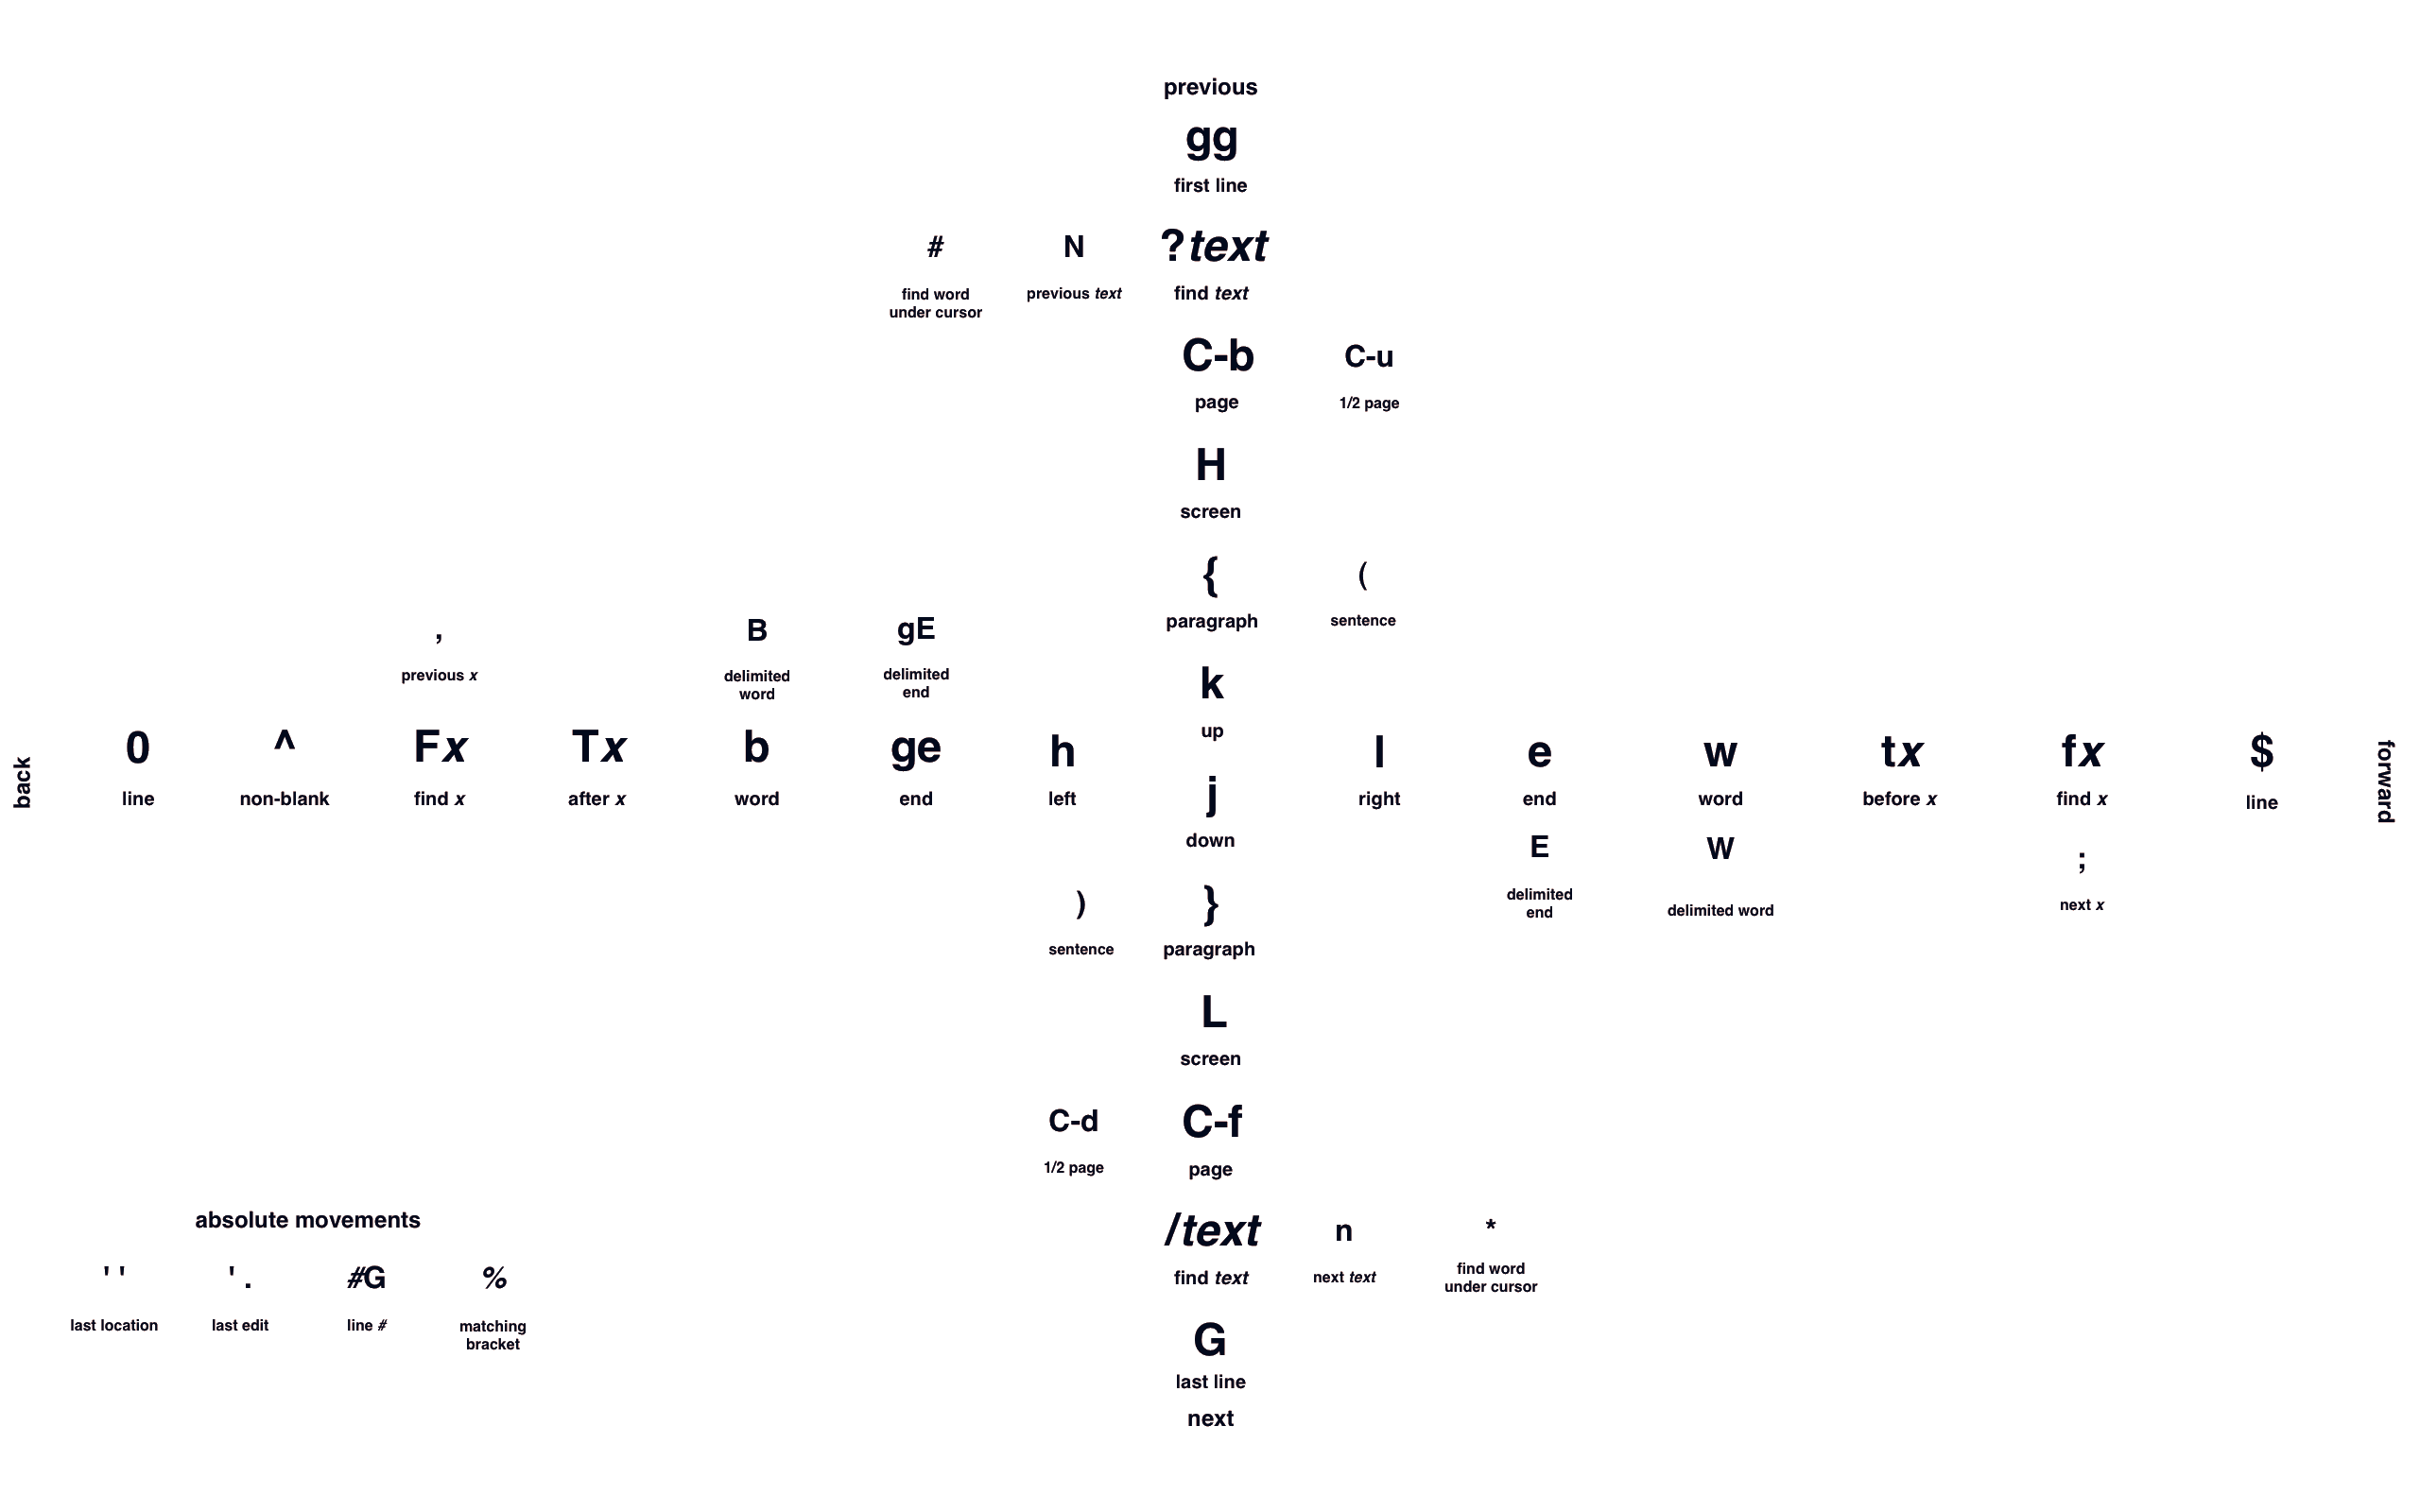
\includegraphics[width=\textwidth]{vim_movements.png}
\end{frame}

\begin{frame}
    \frametitle{Boosted typing (completition)}
    In \viminsert{insert} mode:
    \begin{enumerate}
        \item \viminsert{\vimkey{C-p}}, \viminsert{\vimkey{C-n}} - previous, next autocomplete suggestion
        \item \viminsert{\vimkey{C-x}\vimkey{C-f}} - autocomplete filename (based on cwd)
        \item \viminsert{\vimkey{C-e}}, \viminsert{\vimkey{C-y}} - insert (copy) char from below/above line
    \end{enumerate}
    In \vimnormal{normal} mode:
    \begin{enumerate}
      \item \vimnormal{\vimkey{C-a}}, \vimnormal{\vimkey{C-x}} - increment, decrement number (also hex)\\
        (for operating on dates see tpope/vim-speeddating)
    \end{enumerate}
\end{frame}

\begin{frame}
    \frametitle{Buffers / Windows / Tabs}
    Summary:
    \begin{enumerate}
        \item A \textbf{buffer} is the in-memory text of a file.
        \item A \textbf{window} is a viewport on a buffer.
        \item A \textbf{tab page} is a collection of windows.
    \end{enumerate}
\end{frame}

\begin{frame}
    \frametitle{Buffers / Windows / Tabs: reference topics}
    \begin{itemize} 
        \item \vimhelp{opening-window} (\vimhelp{new}, \vimhelp{split}, \vimhelp{vsplit}) \\
        \item \vimhelp{window-move-cursor} \\
        \item
        \begin{itemize}
            \item \vimnormal{\vimkey{C-w}j} (move left), \vimnormal{\vimkey{C-w}h} (move down), \vimnormal{\vimkey{C-w}l} (move up), \vimnormal{C-w k} (move right)
            \item \vimnormal{\vimkey{C-w}\vimkey{C-w}} (move next)
        \end{itemize}
        \item \vimhelp{window-moving} 
        \item \vimhelp{window-resize}
        \item \vimhelp{buffer-list} 
        \item \vimhelp{list-repeat} (\vimhelp{bufdo}, \vimhelp{windo}, \vimhelp{tabdo})
    \end{itemize}
\end{frame}

\begin{frame}
    \frametitle{Copying and Moving Text}
    \begin{enumerate}
        \item \textbf{"\{a-zA-Z0-9\}} - use register \{a-zA-Z0-9\} for next delete, yank or put (use uppercase character to append with delete and yank)
        \item \textbf{:reg[isters]} - display the contents of all registers
        \item \textbf{["x]y\{motion\}} - yank \{motion\} text [into register x]
        \item \textbf{["x]yy} - yank [count] lines [into register x]
        \item \textbf{["x]Y} - yank [count] lines [into register x] (synonym for yy)
        \item \textbf{\{Visual\}["x]y} - yank the highlighted text [into register x]
        \item \textbf{\{Visual\}["x]Y} - yank the highlighted lines [into register x]
        \item \textbf{:[range]y[ank] [x]} - yank [range] lines [into register x].
        \item \textbf{["x]p}, ["x]P - put the text [from register x] after (for P before)
        \item \textbf{["x]gp}, ["x]gP - just like "p" ("P"), but leave the cursor just after the new text.
        \item \textbf{:[line]pu[t] [x]}, :[line]pu[t]! [x] - put the text [from register x] after (before) [line] (default current line).
    \end{enumerate}
\end{frame}

\begin{frame}
    \frametitle{Undo/Redo/Repeat features}
    \begin{enumerate}
        \item \vimnormal{[count]u}   - undo [count] changes
        \item \vimcommand{:u[ndo]}    - undo one change
        \item \vimnormal{[count]C-R} - redo [count] changes which were undone
        \item \vimcommand{:red[o]}    - redo one change which was undone
        \item \vimnormal{U}          - undo all latest changes on one line.
    \end{enumerate}
    \vimnormal{.} (a dot character) - repeat last change, with count replaced with [count].
    (see sjl/gundo.vim plugin for boosted history navigation)
\end{frame}

\begin{frame}
    \frametitle{Operators and motions}
    In normal mode (\vimnormal{\{operator\}[count]\{motion\}}):
    \begin{enumerate}
        \item - enter an operation (e.g. delete, change, yank, cut)
        \item - provide optional [count] argument
        \item - use a motion (to indicate the text region)
    \end{enumerate}
    Or in visual mode (\vimvisual{[count]\{motion\}\{operator\}}):
    \begin{enumerate}
        \item - provide optional [count] argument
        \item - enter a motion
        \item - use an operation
    \end{enumerate}
\end{frame}

\begin{frame}
    \frametitle{1. Operators}
    \begin{enumerate}
        \item \vimoperator{c}  - change
        \item \vimoperator{d}  - delete
        \item \vimoperator{y}  - yank into register (does not change the text)
        \item \vimoperator{x}  - cut into register
        \item \vimoperator{gu} - make lowercase
        \item \vimoperator{gU} - make uppercase
        \item \vimoperator{!}  - filter through an external program
        \item \vimoperator{=}  - filter through equalprg or C-indenting if empty
        \item \vimoperator{gq} - text formatting
        \item \vimoperator{g?} - ROT13 encoding aka boss mode
    \end{enumerate}
\end{frame}

\begin{frame}
    \frametitle{2. Left-right motions \vimhelp{left-right-motions}}
    \begin{itemize}
        \item \vimmotion{h}, \vimmotion{\vimkey{Left}}, \vimmotion{\vimkey{C-h}}, \vimmotion{\vimkey{BS}} - [count] characters to the left
        \item \vimmotion{l}, \vimmotion{\vimkey{Right}}, \vimmotion{\textless{}Space\textgreater{}} - [count] characters to the right
        \item \vimmotion{0}, \vimmotion{\textless{}Home\textgreater{}} - to the first character of the line
        \item \vimmotion{f\{char\}} - to [count]th occurrence of \{char\} to the right.\\ The cursor is placed on \{char\} inclusive
        \item \vimmotion{F\{char\}} - to the [count]'th occurrence of \{char\} to the left. The cursor is placed on \{char\} exclusive.
        \item \vimmotion{t\{char\}} - till before [count]'th occurrence of \{char\} to the right. The cursor is placed on the character left of \{char\} inclusive.
        \item \vimmotion{T\{char\}} - till after [count]'th occurrence of \{char\} to the left. The cursor is placed on the character right of \{char\} exclusive.
        \item \vimmotion{;} - repeat latest f, t, F or T [count] times
        \item \vimmotion{,} - repeat latest f, t, F or T in opposite direction [count] times
    \end{itemize}
\end{frame}

\begin{frame}
    \frametitle{3. Up-down motions \vimhelp{up-down-motions}}
    \begin{itemize}
        \item \vimmotion{k}, \vimmotion{\textless{}Up\textgreater{}}, \vimmotion{C-p} - [count] lines upward (linewise)
        \item \vimmotion{j}, \vimmotion{\textless{}Down\textgreater{}}, \vimmotion{C-j}, \vimmotion{C-n} - [count] lines downward (linewise)
        \item \vimmotion{gk}, \vimmotion{g\textless{}Up\textgreater{}} - [count] display-wise lines upward (useful when lines are wrapped)
        \item \vimmotion{gj}, \vimmotion{g\textless{}Down\textgreater{}} - [count] display-wise lines downward (useful when lines are wrapped)
        \item \vimmotion{G} - goto line, default first line
        \item \vimmotion{\textless{}C-End\textgreater{}} - goto line [count], default last line
        \item \vimmotion{\textless{}C-Home\textgreater{}}, \vimmotion{gg} - goto line [count], default first line, on the first non-blank character
        \item \vimmotion{:[range]} - set the cursor on the last line number in [range]
        \item \vimmotion{N\%} - go to \{count\} percentage in the file
    \end{itemize}
\end{frame}

\begin{frame}
    \frametitle{4. Word motions \vimhelp{word-motions}}
    \begin{itemize}
      \item \vimmotion{w}                               - [count] words forward.  (exclusive)
      \item \vimmotion{W}, \vimmotion{\vimkey{C-Right}} - [count] WORDS forward.  (exclusive)
      \item \vimmotion{e}                               - forward to the end of word [count] (inclusive)
      \item \vimmotion{E}                               - forward to the end of WORD [count] (inclusive)
      \item \vimmotion{\vimkey{S-Left}}, \vimmotion{b}  - [count] words backward.  (exclusive)
      \item \vimmotion{\vimkey{C-Left}}, \vimmotion{B}  - [count] WORDS backward.  (exclusive)
      \item \vimmotion{ge}                              - backward to the end of word [count] (inclusive)
      \item \vimmotion{gE}                              - backward to the end of WORD [count] (inclusive)
    \end{itemize}
    {\footnotesize 
    A word consists of a sequence of letters, digits and underscores, or a
    sequence of other non-blank characters, separated with white space (spaces,
    tabs, EOL). A WORD consists of a sequence of non-blank characters, separated with white
    space.}
\end{frame}

\begin{frame}
    \frametitle{5. Text object motions \vimhelp{object-motions}}
    \vimhelp{text-objects} 
    \begin{itemize}
      \item \vimmotion{(} - [count] sentences backward (exclusive)
      \item \vimmotion{)} - [count] sentences forward (exclusive)
      \item \vimmotion{\{} - [count] paragraphs backward (exclusive)
      \item \vimmotion{\}} - [count] paragraphs forward (exclusive)
      \item \vimmotion{]]} - [count] sections forward or to the next '\{' in the first column.When used after an operator, then also stops below a '\}' in the first column (exclusive)
      \item \vimmotion{][} - [count] sections forward or to the next '\}' in the first column (exclusive)
      \item \vimmotion{[[} - [count] sections backward or to the previous '\{' in the first column (exclusive)
      \item \vimmotion{[]} - [count] sections backward or to the previous '\}' in the first column (exclusive)
    \end{itemize}
\end{frame}

\begin{frame}
    \frametitle{6. Text object selection \vimhelp{object-select}}
    \begin{itemize}
        \item \vimmotion{aw} - "a word", select [count] words (see (\textrm(*word*))
        \item \vimmotion{aW} - "a WORD", select [count] WORDs (see (\textrm(*WORD*))
        \item \vimmotion{as} - "a sentence", select [count] sentences (see (\textrm(*sentence*))
        \item \vimmotion{ap} - "a paragraph", select [count] paragraphs (see (\textrm(*paragraph*))
        \item \vimmotion{a]}, \vimmotion{a[} - "a [] block", select [count] '[' ']' blocks
        \item \vimmotion{a)}, \vimmotion{a(}, \vimmotion{ab} - "a block", select [count] blocks
        \item \vimmotion{a\textgreater{}}, \vimmotion{a\textless{}} - "a \textless{}\textgreater{} block", select [count] \textless{}\textgreater{} blocks
        \item \vimmotion{at} - "a tag block", select [count] tag blocks
        \item \vimmotion{a"}, \vimmotion{a'}, \vimmotion{a`} - "a quoted string"
    \end{itemize}
\end{frame}

\begin{frame}
    \frametitle{6. Text object selectionv \vimhelp{object-select}}
    (inner variants)
    \begin{itemize}
        \item \vimmotion{iw}                                 - "inner word", select [count] words (\textrm{*word*})
        \item \vimmotion{iW}                                 - "inner WORD", select [count] WORDs (see (\textrm(*WORD*))
        \item \vimmotion{is}                                 - "inner sentence", select [count] sentences (see (\textrm(*sentence*))
        \item \vimmotion{ip}                                 - "inner paragraph", select [count] paragraphs (see (\textrm(*paragraph*))
        \item \vimmotion{i]}, \vimmotion{i[}                 - "inner [] block", select [count] '[' ']' blocks
        \item \vimmotion{i)}, \vimmotion{i(}, \vimmotion{ib} - "inner block", select [count] blocks
        \item \vimmotion{i\textless}, \vimmotion{i\textgreater} - "inner \textless\textgreater block", select [count] \textless\textgreater blocks
        \item \vimmotion{it}                                 - "inner tag block", select [count] tag blocks
        \item \vimmotion{i"}, \vimmotion{i'}, \vimmotion{i`} - like a", a' and a`, but exclude the quotes
    \end{itemize}
\end{frame}

\begin{frame}[fragile]
    \frametitle{7. Marks \vimhelp{mark-motions}}
    \begin{itemize}
        \item \vimnormal{m\{a-zA-Z\}}                                - set mark \{a-zA-Z\} at cursor position (does not move the cursor, this is not a motion command).
        \item \vimnormal{\'{}\{a-z\}}, \vimnormal{\`{}\{a-z\}}       - jump to the mark \{a-z\} in the current buffer.
        \item \vimnormal{\'{}\{A-Z0-9\}}, \vimnormal{\`{}\{A-Z0-9\}} - jump to the mark \{A-Z0-9\} in the file where it was set
    \end{itemize}
    Jump to last marks:
    \begin{itemize}
        \item \vimnormal{\`{}\`{}} - jump to the specified location (motion is exclusive)
        \item \vimnormal{\'{}\'{}} - jump to the first non-blank character in the line of the specified location (motion is linewise)
    \end{itemize}
\end{frame}

\begin{frame}
    \frametitle{Macros}
    \begin{enumerate}
        \item \vimnormal{qa} - start recording to register \textbf{a}
        \item series of commands to be recorded
        \item \vimnormal{q} stop recording (being in a normal mode)
    \end{enumerate}
    \begin{itemize}
        \item \vimnormal{@a} - execute macro (from register \textbf{a})
        \item \vimnormal{@@} - execute macro again
        \item \vimcommand{:g/pattern/normal @a} - execute macro for given range
    \end{itemize}
\end{frame}

\begin{frame}
    \frametitle{vimdiff - Use vim to compare files}
    \begin{enumerate}
      \item Command line interface (maybe used together with git/svn)\\
        \texttt{\$ vimdiff file1 file2}
      \item Start comparing within vim:
          \begin{itemize}
            \item \vimcommand{:diffthis} $\rightarrow$ \vimcommand{:sp file2} $\rightarrow$ \vimcommand{:diffthis}
            \item \vimcommand{:diffoff} - turn off comparison on a file
            \item \vimcommand{:[range]diffget} - insert from other file
            \item \vimcommand{:[range]diffput} - insert into other file
          \end{itemize}
    \end{enumerate}
\end{frame}

\begin{frame}
    \frametitle{Search}
    \vimnormal{/pattern\vimkey{CR}} (start search) $\rightarrow$ \vimnormal{n} or \vimnormal{/\vimkey{CR}} - next, \vimnormal{N} - previous\\
    \vimcommand{:[range]/pattern} - to use within range
    \begin{itemize}
        \item regex rules:
        \begin{itemize}
            \item \vimcommand{\textbackslash{(}} - \vimcommand{\textbackslash{)}} - groups
            \item \vimcommand{.} - any character
            \item \vimcommand{*} - any number of repetition (0+)
            \item \vimcommand{?} - optional (0 or 1)
            \item \vimcommand{+} - positive number of repetition (1+)
            \item \vimcommand{\textbackslash{s}}, \vimcommand{\textbackslash{d}}, \vimcommand{\textbackslash{w}}, \vimcommand{\textbackslash{a}} - whitespace, digit, word, alpha characters
            \item \vimcommand{\string^}, \vimcommand{\$} - begin of line, end of outline
            \item \vimcommand{\textbackslash{\textless}}, \vimcommand{\textbackslash{\textgreater}} - begin, end of word
            \item \vimcommand{[\string^XYZ]} - exclude characters XYZ
        \end{itemize}
        \item \vimcommand{:set hlsearch} - enable search result highlighting
        \item \vimcommand{:set incsearch} - search while typing (incremental)
        \item If needed: \vimcommand{:nohl} to disable highlighting afterwards
    \end{itemize}
\end{frame}

\begin{frame}
  \frametitle{Power of g (global command)}
  \vimcommand{:[range]g/pattern/cmd}

  \begin{itemize}
    \item Delete all lines matching a pattern: \vimcommand{:g/pattern/d}
    \item Delete all lines that do not match a pattern: \vimcommand{:g!/pattern/d} or \vimcommand{:v/pattern/d}
    \item Delete all blank lines: \vimcommand{:g/\string^\textbackslash{s}*\$/d}
    \item Copy all lines matching a pattern to end of file: \vimcommand{:g/pattern/t\$}
    \item Move all lines matching a pattern to end of file: \vimcommand{:g/pattern/m\$}
    \item Copy all lines matching a pattern to register 'a'. \vimnormal{qaq}\vimcommand{:g/pattern/y A} (clearing register first)
    \item Run a macro on matching lines (example assuming a macro recorded as 'q'): \vimcommand{:g/pattern/normal @q}
    \item Call custom command on match \vimcommand{:g/pattern/\textbackslash{=}call foo()}
  \end{itemize}
\end{frame}

\begin{frame}
    \frametitle{Search and replace substitutions}
    Common syntax (allows custom separators e.g. \vimcommand{/}, \vimcommand{\#}, \vimcommand{\$}, \vimcommand{,}):
    {\footnotesize 
    \begin{itemize}
        \item \vimcommand{:[range]s/pattern/replace/flags}
        \item \vimcommand{:s/pattern/replace/flags} - within line
        \item \vimcommand{:\%s/pattern/replace/flags}
        \item \vimcommand{:\%s,pattern,replace,flags}
    \end{itemize}
    }
    Where
    \begin{itemize}
        \item pattern supports regex (only grouping needs escaping):\\
          \vimcommand{\textbackslash{(}}, \vimcommand{\textbackslash{)}}, \vimcommand{.}, \vimcommand{*}, \vimcommand{?}, \vimcommand{+}, \vimcommand{[\string^X]}
        \item in replace use groups with \vimcommand{\textbackslash{1}}, \vimcommand{\textbackslash{2}}, \ldots or whole match \vimcommand{\&}
        \item flags: \vimcommand{g} (global), \vimcommand{c} (confirm), \vimcommand{i} (ignore case)
        \item call custom command on match {\footnotesize \vimcommand{\textbackslash{=}call eval\_replacement()}}
        \item use nested replace \vimcommand{\textbackslash{=}substitute()} with \vimcommand{submatch()}, e.g.:
    {\footnotesize 
          \vimcommand{:s/outer/\textbackslash{=}substitute(submatch(0), 'inner', 'replace', 'g')}
    }
        \item use nested replace with \vimcommand{:g}, e.g.: \vimcommand{:g/good/s/bad/ugly/g}
    \end{itemize}
\end{frame}

\begin{frame}
    \frametitle{Shell invocation}
    \begin{itemize}
      \item \vimcommand{:read !ls -la} or \vimcommand{:read !date}
      \item \vimcommand{:\%!sort}\
      \item \vimcommand{:let curdate=system('date')}
      \item backticks \vimcommand{:new `date`}
    \end{itemize}
\end{frame}

\begin{frame}
    \frametitle{Command mode}
    \begin{itemize}
        \item know how to work with ctrl+r
        \item use the marked region as default substitute pattern
    \end{itemize}
\end{frame}

\section{PLUGINS}
\begin{frame}
    \frametitle{vundle}
    \begin{itemize}
        \item easy way to manage
        \item clean and readable vimrc
        \item rule of thumb: extract your config and store it as a plugin on github
    \end{itemize}
\end{frame}

\begin{frame}
    \frametitle{nerdtree, vim-nerdtree-tab, nerdtree-toggle, vim-rooter}
    \begin{itemize}
        \item Navigate through filesystem,
        \item Allows open, open split h/v, open tab, quick preview,
        \item Support for bookmarks.
        \item :NERDTreeFind
        \item  plugin nerdtree-tabs keeps nerd tree toggle accross all tabs
    \end{itemize}
 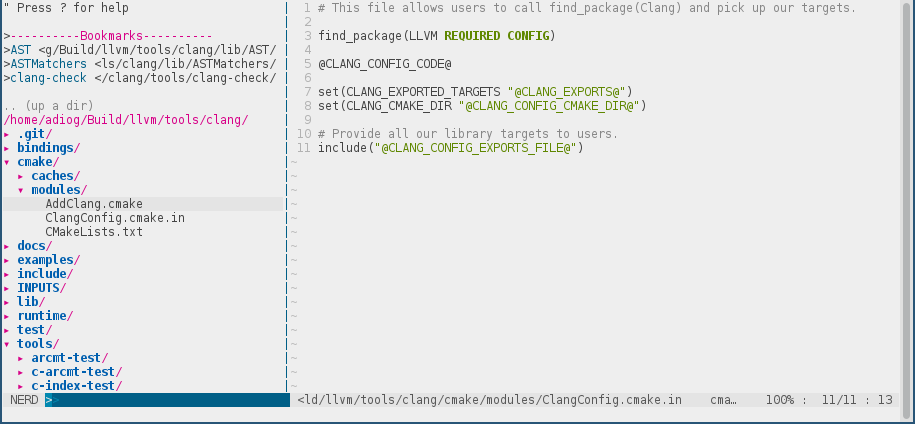
\includegraphics[scale=0.33]{vim_nerdtree_example.png}\\
\end{frame}

\begin{frame}
  \frametitle{YouCompleteMe}
    works ok with --system-clang (still recommend clion as default)
    have not checked carefully the rope variant, but it seemed also ok (still recommend pycharm)
\end{frame}

\begin{frame}
  \frametitle{tagbar}
 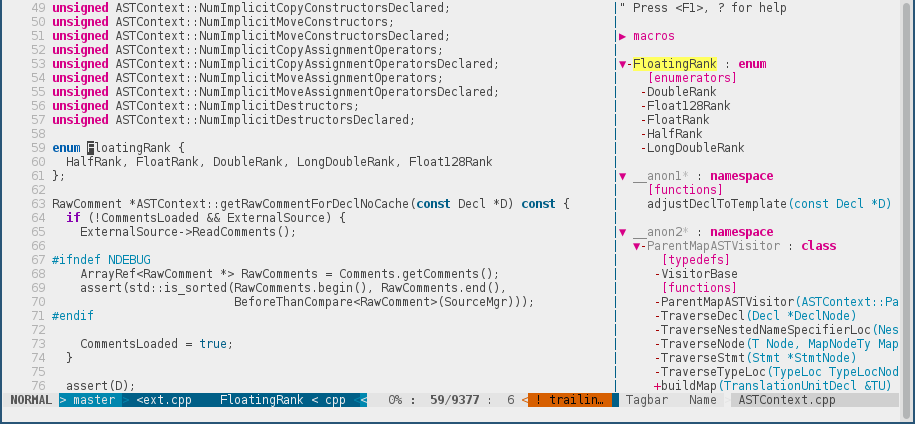
\includegraphics[scale=0.33]{vim_tagbar_example.png}\\
\end{frame}

\begin{frame}
  \frametitle{undotree}
  visualize (with diff) and navigate through the history of file changel
 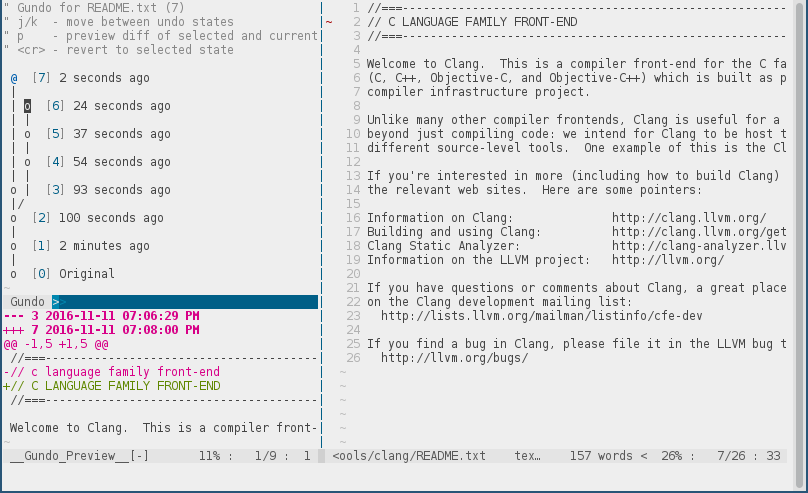
\includegraphics[scale=0.33]{vim_undotree_example.png}\\
\end{frame}

\begin{frame}
  \frametitle{git-gutter}
  git mark modified lines (useful)
\end{frame}

\begin{frame}
  \frametitle{fugitive}
  git facilities
\end{frame}

\begin{frame}[fragile]
  \frametitle{tabular}
{\footnotesize
\begin{verbatim}
| column | column|
row | value | value|
other row | other value | yet another value |
\end{verbatim}
}
\vimcommand{:\%Tabularize /|}
{\footnotesize
\begin{verbatim}
          | column      | column            |
row       | value       | value             |
other row | other value | yet another value |
\end{verbatim}
}
\end{frame}

\begin{frame}
  \frametitle{airline}
\end{frame}

\begin{frame}
  \frametitle{vim-slime}
  useful to trigger external commands
\end{frame}


\begin{frame}
  \frametitle{abolish}
\end{frame}

\begin{frame}[fragile]
    \frametitle{Abbreviations and hiding text}
    \begin{itemize}
      \item \vimcommand{:iab tte text\_to\_expand} - define 'tte' abbreviation
        \item Conceal known chars outside currently edited line:\\
 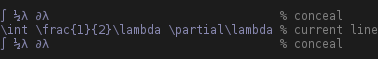
\includegraphics[scale=0.6]{vim_conceal_example.png}\\
\textrm{Below sample config:}
{\footnotesize
\begin{verbatim}
if has('conceal')
  let g:tex_conceal="adgms"
  set conceallevel=2
  highlight! link Conceal texMathSymbol
endi

syn match texMathSymbol '\\alpha\>' contained conceal cchar=αA
syn match texMathSymbol '\\beta\>' contained conceal cchar=βB
syn match texMathSymbol '\\gamma\>' contained conceal cchar=γG
\end{verbatim}
}
    \end{itemize}
\end{frame}

\begin{frame}
    \frametitle{Expressions register}
    In \viminsert{\vimmode{insert}} mode:
    \begin{enumerate}
        \item \viminsert{\textless{}C-r\textgreater{}=}
        \item enter VimScript command to be evaluated
    \end{enumerate}
    This can be used as a in place calculator, e.g. on line:\\
    \textrm{6 * 7 =}\\
    the following sequence may be used to append a result:\\
    \vimnormal{0vt="ayA\textless{}C-r\textgreater{}=\textless{}C-r\textgreater a\textless{}CR\textgreater}
\end{frame}

\begin{frame}
    \frametitle{colorschemes / cursorcolumn line / hexhighlight}
    tricks:i
    \begin{itemize}
        \item    rotate over all color schemes
        \item pick the name of current text segment
        \item set the color for custom element
        \item display the html color format \#156123 with real color
    \end{itemize}
\end{frame}

\begin{frame}
    \frametitle{Spellchecker}
    \begin{itemize}
        \item \vimcommand{:setlocal spell spelllang=en\_us} to set language (e.g. )
        \item \vimcommand{:set spell} to enable spellchecker
        \item \vimnormal{]s} Move to next misspelled word after the cursor.
        \item \vimnormal{[s} Like "]s" but search backwards.
        \item \vimnormal{z=} For the word under/after the cursor suggest correctly spelled words. This also works to find alternatives for a word that is not highlighted as a bad word, e.g., when the word after it is bad.
    \end{itemize}
    additional features: add words to dictionary etc.
\end{frame}

\begin{frame}
    \frametitle{Folds}
    \begin{itemize}
        \item \vimnormal{zf\{motion\}}, \vimvisual{\{visual\}zf} Operator to create a fold.  This only works when 'foldmethod' is "manual" or "marker".  The new fold will be closed for the "manual" method.  'foldenable' will be set.
        \item \vimcommand{:[range]fo[ld]} Create a fold for the lines in {range}.  Works like "zf".
        \item \vimnormal{zd} - delete one fold at the cursor.
        \item \vimnormal{zo} - open one fold under the cursor.
        \item \vimnormal{zO} - open all folds under the cursor recursively.
        \item \vimnormal{zc} - close one fold under the cursor.
        \item \vimnormal{zC} - close all folds under the cursor recursively.
    \end{itemize}
\end{frame}

\begin{frame}
    \frametitle{Other features}
    \begin{itemize}
        \item list number
        \item built in autocomplete / no prob with connecting external tools
        \item topics to cover:
        \item context autocomplete
        \item inplace static source code analyser
    \end{itemize}
\end{frame}

\begin{frame}
    \frametitle{Remaining issues}
    \begin{itemize}
        \item vimrc / recommended setup / mappings vimscript basic (function declaration / scopes / if / types / )
        \item  (sort)
        \item    os interaction (in place edit)
        \item   external indent
    \end{itemize}
\end{frame}

\begin{frame}
    \frametitle{Useful links}
    \begin{itemize}
        \item http://vimcasts.org
        \item http://vimgolf.org
        \item http://vimregex.com
        \item https://github.com/tpope
        \item http://learnvimscriptthehardway.stevelosh.com/
        \item https://github.com/vim/vim
        \item https://github.com/vim-scripts
        \item http://vim.org
        \item https://neovim.io
        \item https://github.com/neovim/neovim
    \end{itemize}
\end{frame}

\end{document}



%            \begin{verbatim}
%            *m* *mark* *Mark*
%            m\{a-zA-Z\}     Set mark \{a-zA-Z\} at cursor position (does not move
%      the cursor, this is not a motion command).
%
%      '\{a-z\}  `\{a-z\}        Jump to the mark \{a-z\} in the current buffer.
%
%
%            *'A* *'0* *`A* *`0*
%            '\{A-Z0-9\}  `\{A-Z0-9\}    To the mark \{A-Z0-9\} in the file where it was set (not
%      a motion command when in another file).  \{not in Vi\}
%      marks 
%      
%      
%      :reg[isters] \{arg\}  Display the contents of the numbered and named
%      registers that are mentioned in \{arg\}.  For example:
%        :dis 1a
%      to display registers '1' and 'a'.  Spaces are allowed
%      in \{arg\}.  \{not in Vi\}
%      :di[splay] [arg]  Same as :registers.  \{not in Vi\}
%      ["x]y\{motion\}       Yank \{motion\} text [into register x].  When no
%      characters are to be yanked (e.g., "y0" in column 1),
%      this is an error when 'cpoptions' includes the 'E'
%      flag.
%      ["x]yy            Yank [count] lines [into register x] |linewise|.
%      ["x]Y         yank [count] lines [into register x] (synonym for
%      yy, |linewise|).  If you like "Y" to work from the
%      cursor to the end of line (which is more logical,
%      but not Vi-compatible) use ":map Y y\$".
%      \{Visual\}["x]y       Yank the highlighted text [into register x] (for
%      \{Visual\} see |Visual-mode|).  \{not in Vi\}
%      \{Visual\}["x]Y       Yank the highlighted lines [into register x] (for
%      \{Visual\} see |Visual-mode|).  \{not in Vi\}
%      :[range]y[ank] [x]    Yank [range] lines [into register x].
%      :[range]y[ank] [x] \{count\}
%      Yank \{count\} lines, starting with last line number
%      in [range] (default: current line |cmdline-ranges|),
%      [into register x].
%      ["x]p         Put the text [from register x] after the cursor
%      [count] times.  \{Vi: no count\}
%      ["x]P         Put the text [from register x] before the cursor
%      [count] times.  \{Vi: no count\}
%      ["x]<MiddleMouse> Put the text from a register before the cursor [count]
%      times.  Uses the "* register, unless another is
%      specified.
%      Leaves the cursor at the end of the new text.
%      Using the mouse only works when 'mouse' contains 'n'
%      or 'a'.
%      \{not in Vi\}
%      If you have a scrollwheel and often accidentally paste
%      text, you can use these mappings to disable the
%      pasting with the middle mouse button:
%        :map <MiddleMouse> <Nop>
%        :imap <MiddleMouse> <Nop>
%      You might want to disable the multi-click versions
%      too, see |double-click|.
%      ["x]gp            Just like "p", but leave the cursor just after the new
%      text.  \{not in Vi\}
%      ["x]gP            Just like "P", but leave the cursor just after the new
%      text.  \{not in Vi\}
%  \end{verbatim}
%

%let g:I=1
%g/^- id: \d\+$/ s/\d\+/\=g:I/|let g:I=g:I+1

%:.+1,$g/^- id: \d\+$/normal! 0^A


